\chapter{Credit mining Implementation and Experimental Setup}
\label{chp:implexperiment}
In the previous chapter, we discussed how the credit mining system was designed. In this chapter, we show how credit mining system is implemented in Tribler, a python torrent client that was built at the Delft University of Technology. Based on this implementation, we come up with the suitable experiment design to answer our research question in the previous chapter. 

This chapter consists of the elaboration of both implementation and its experiment execution plan. First, in section \ref{section:triblerintregration}, we will describe how the credit mining system is implemented within Tribler. As an open source project, Tribler has a guideline for a new submodule that will be integrated. We comply to that guideline as we will describe later. To evaluate the system, we introduce \textit{gumby} on section \ref{section:gumby}, the experiment runner developed by in-house Tribler team. The section \ref{section:cmexp} will follow to explain the actual experiment setup plan. We will elaborate the environment condition and code alteration regarding the experiment that need to be fulfilled.

\section{Tribler integration}
\label{section:triblerintregration}
As a proof of concept, credit mining system was implemented as a module in Tribler. Tribler was built using python, compatible with version 2.x and 3.x. At the time credit mining system implemented in Tribler, Tribler still use WX as GUI (Graphical User Interface) framework. As for the future, Tribler will move its GUI to use Qt starting version 7.0 onwards. All of those components made Tribler work cross platform (Linux, MacOS, and Windows).

In the prior work, some of the credit mining system code were implemented by \citeauthor{2015:creditmining:capota} and Egbert Bouman in his Tribler fork\footnote{\url{https://github.com/mihaic/tribler/tree/channel_boosting_new_exp}} instead of the main repository. This made the compatibility and stability between Tribler and credit mining system broke, thus make the system unusable. At this point, the credit mining code was 1528 line long with 51 deletions compared to the main branch.

% implemented in wx for GUI
\subsection{Contribution on software engineering}
As part of the software engineering process, the credit mining code needs to pass several steps before merged into main repository. In Tribler, there are two main branches, which are \texttt{devel} for all new features and fixes, and \texttt{next} which contains bug fixes for the stable release. The first credit mining prototype was directed to \texttt{devel} branch as it is a new feature at that point. Before it can be merged, the code must pass the peer review and unit tests on Jenkins\footnote{\url{http://jenkins.tribler.org/}}. This process is repeated until there are no other feedbacks. As shown in Figure \ref{fig:cmpullrequest}, the first credit mining prototype was heavily discussed by 6 other participants and more than 450 comments. It also takes almost 3 months to accommodate all the feedbacks and reviews. The contributions of this integration worth more than 4200 added lines and 140 deletions. The code portion is quite balanced with 1425 lines goes to GUI part of the code, 1290 lines to the credit mining system itself, 1160 lines to the tests, and the rest to other Tribler components to accommodate credit mining system. At the time of merging it has passed the necessary code coverage and allowed number of violations. Therefore, it confirms that credit mining system can be deployed in all system that supported by Tribler. 

\begin{figure}[h]
	\centering
	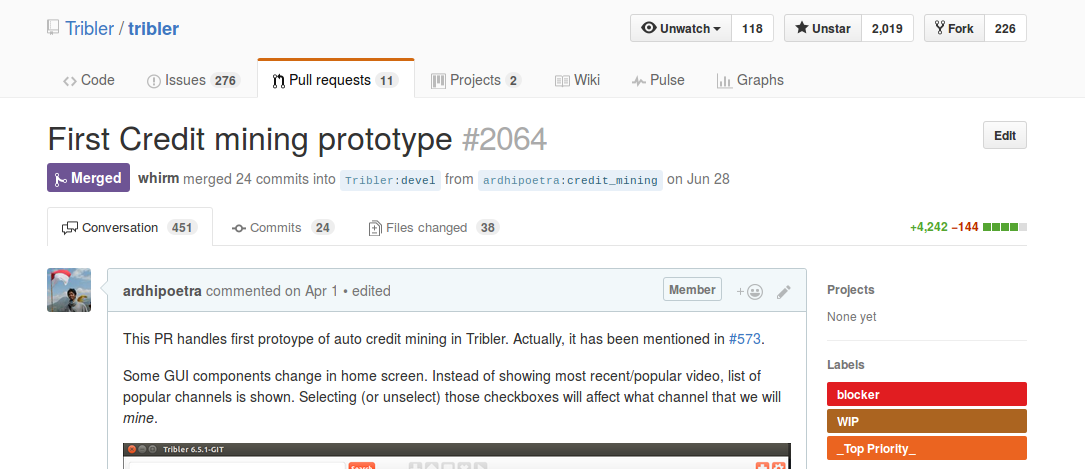
\includegraphics[width=\textwidth]{pics/cm_pr_crop.png}
	\caption[Merged pull request on credit mining prototype]{Merged pull request on credit mining prototype\footnotemark.}
	\label{fig:cmpullrequest}
\end{figure}
\footnotetext{Available in : \url{https://github.com/Tribler/tribler/pull/2064/}}

To ensure the quality of the main branch, any code submitted through pull request is tested by a unit test mechanism. There are two categories in the credit mining unit tests. First one is the tests that check its basic function such as policies, peer translation, RSS parser, similarity function, and mining configuration along with its dependencies. It also tests for the unwanted/error case and how credit mining system will react. The second test is more complex because it emulates the whole credit mining flow for each mining source type. For RSS source, the test deployed local server acting as RSS feeder. As for \textit{channel} source, the test suite prepares the environment by fabricating both local channel and torrent, inserting torrent metadata into \textit{channel}, and pushing created channel to \textit{AllChannelCommunity}. 

\subsection{Graphical user interface revampment}
\begin{figure}[h]
	\centering
	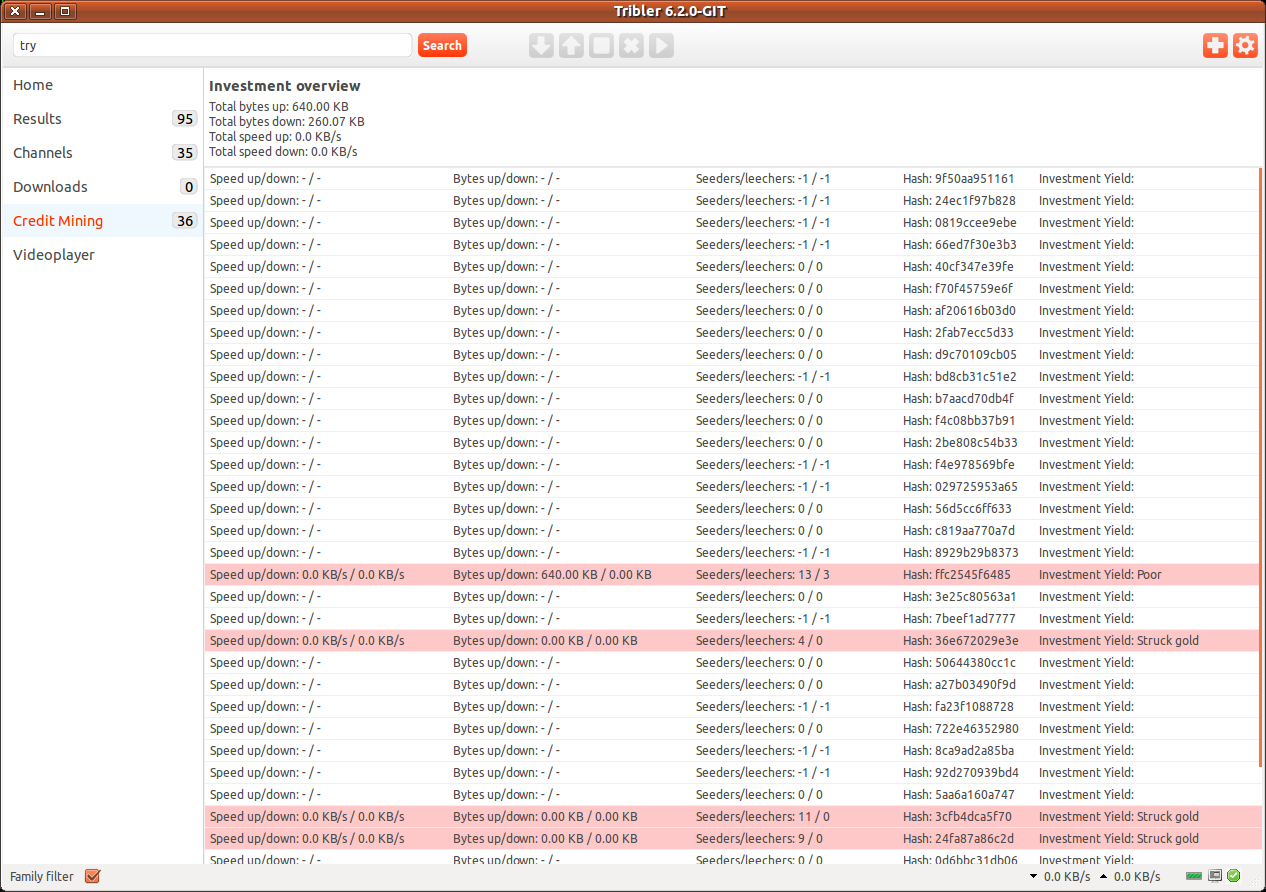
\includegraphics[width=0.8\textwidth]{pics/old_cm.png}
	\caption{The GUI for showing information from prior work \cite{2015:creditmining:capota}.}
	\label{fig:oldcm}
\end{figure}
In the prior version, it was not possible to add the mining sources except changing from the Tribler configuration file. There are also several limitations such as incompatible source and instability. Figure \ref{fig:oldcm} shows the only interface available from the previous work. As for our work, the credit mining main screen shown in \ref{fig:overview}. We improved the investment summary by adding more mining source information. In the same window, we also integrated an interface to easily add or remove mining sources. Adding RSS and directory source can be done by clicking the upper left option. This action will trigger a popup window like shown in Figure \ref{fig:overview}. Adding \textit{channel} as a source can be done by put the mark in the check boxes in the channel list.

\begin{figure}[h!]
	\begin{adjustwidth}{-1.5cm}{-1cm}
%		\begin{subfigure}[t]{0.8\textwidth}
			\centering
			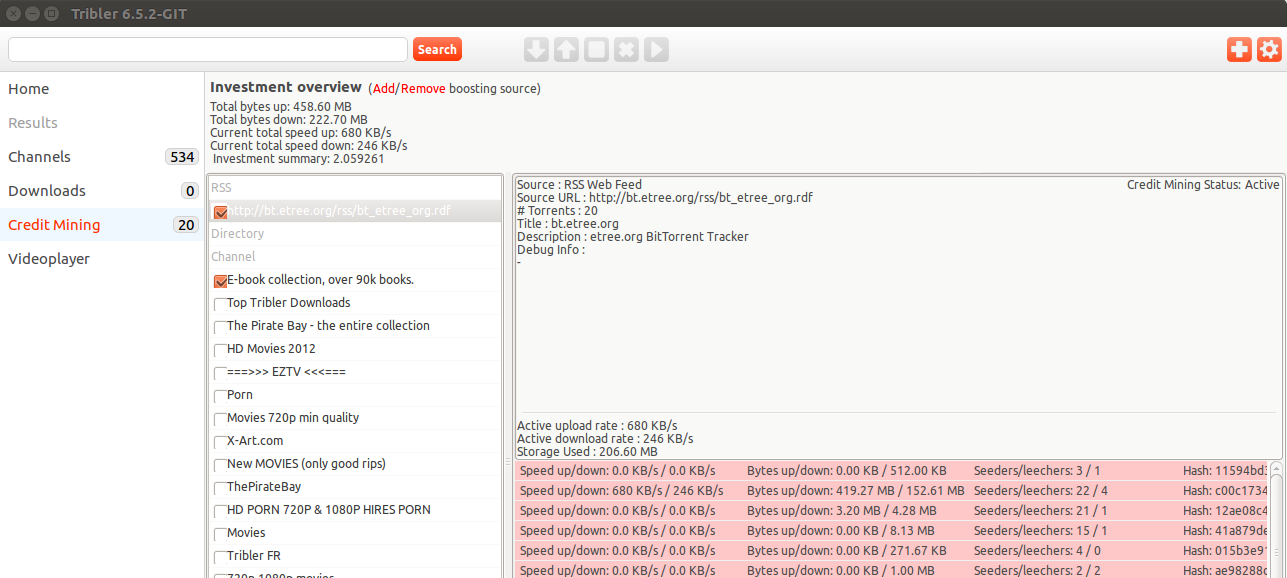
\includegraphics[width=1.2\textwidth]{pics/overview_result.png}
			\caption{Credit mining main window with adding new source.}
			\label{fig:overview}
%		\end{subfigure}
%		~
%		\begin{subfigure}[t]{0.6\textwidth}
%			\centering
%			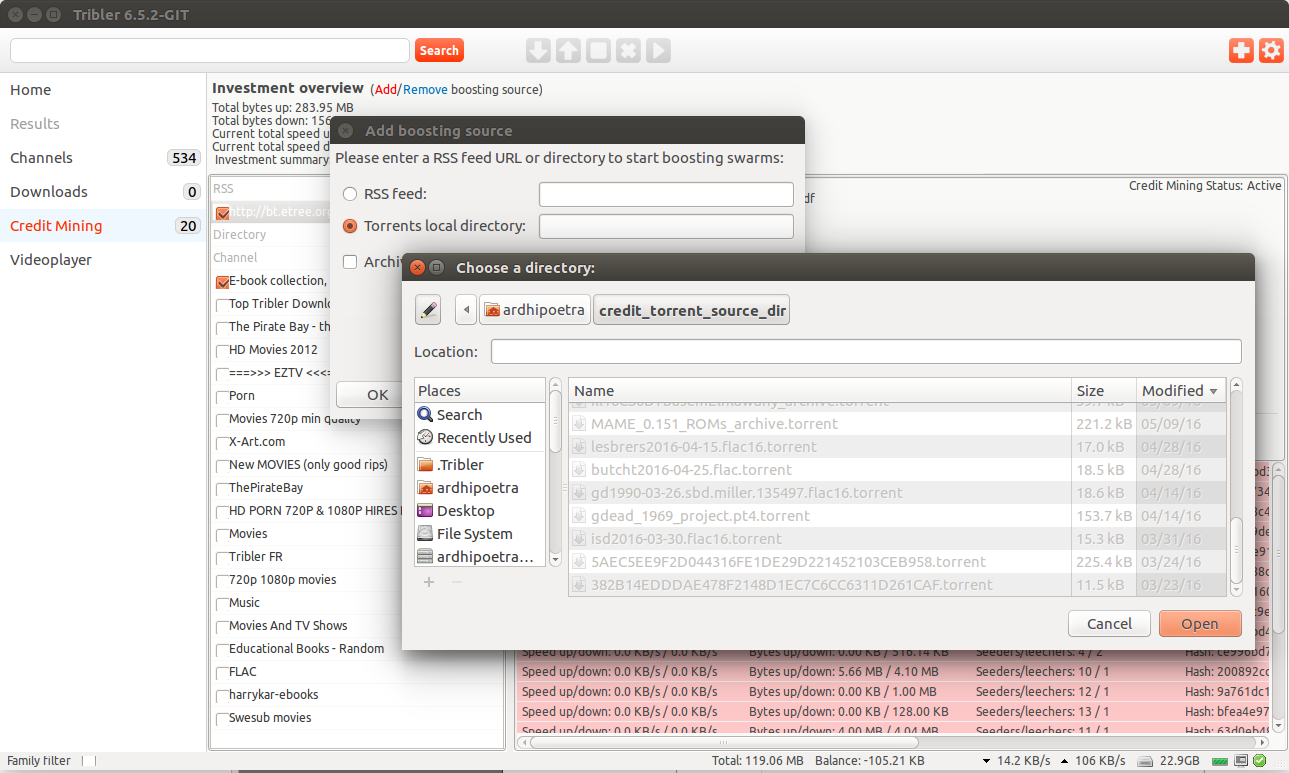
\includegraphics[width=\textwidth, height=6cm]{pics/add_source.png}
%			\caption{The interface of adding mining source.}
%			\label{fig:addsource}
%		\end{subfigure}
		
	\end{adjustwidth}
\end{figure}

As an experimental feature, credit mining system is disabled by default in Tribler. Activating credit mining module made the home screen of Tribler changed. We put several channels sorted by its popularity at the home screen as shown in Figure \ref{fig:homecm}. The purpose is to encourage user to altruistically mine. To show the channel information, we provide two details. First is the popularity, which shown by the number of stars. Second is random swarm that resides within a particular channel. A user can simply click which channel he want to mine either on this screen or the credit mining main screen. Both actions will also be reflected on the other screen. 

\begin{figure}[h]
	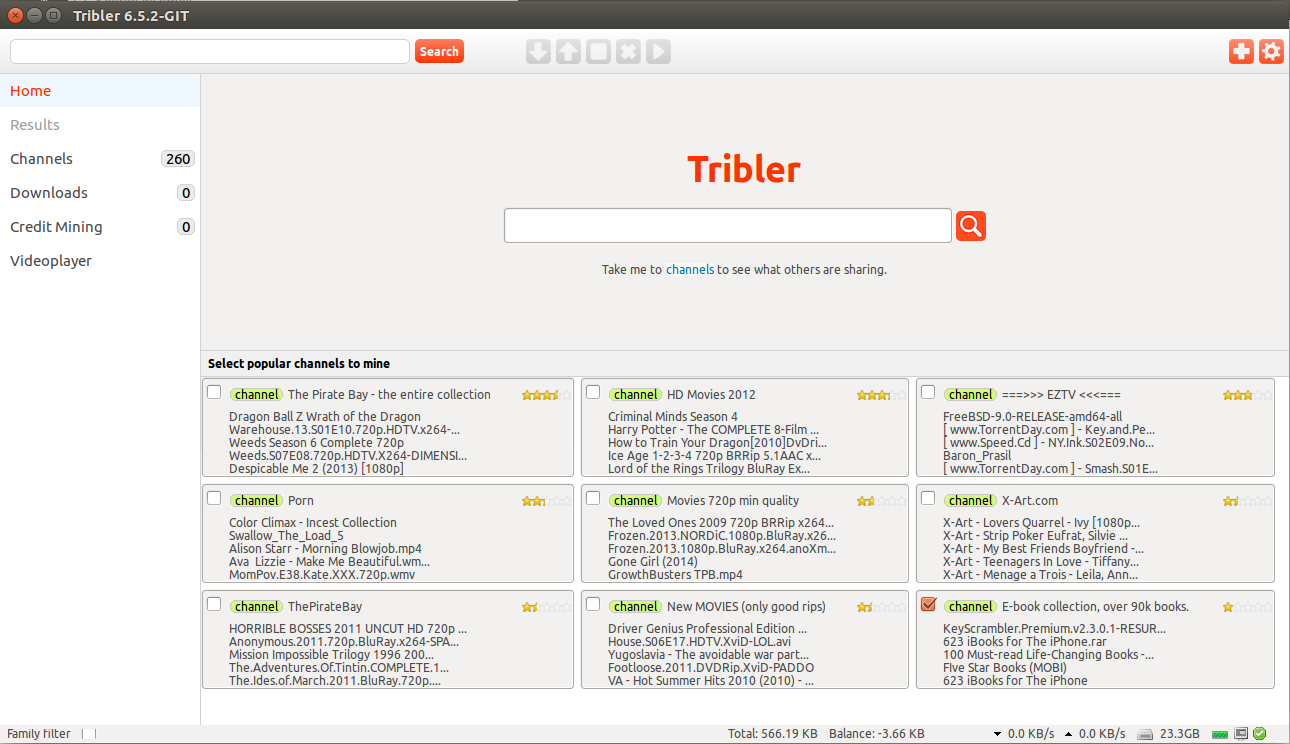
\includegraphics[width=\textwidth]{pics/home_channel.png}
	\caption{The home interface of Tribler with credit mining active.}
	\label{fig:homecm}
\end{figure}

%\todo[inline]{Add stuff}
\section{Gumby}
\label{section:gumby}
\textit{Gumby}\footnote{\url{https://github.com/Tribler/gumby}} is an experiment runner framework for both Tribler and Dispersy. Gumby can run on both local computer and cluster computer to emulate the experiment. Gumby runs on different scenarios, which consists of many commands, for each experiment. It also uses a configuration file to define all the settings needed for running the experiment. The developer can easily specify the number of peers needed, the post process script after running the experiment, the value that needed to be distributed to all of the peers, and many others. The most important part is to code the \textit{client} that written in \texttt{python}. In \textit{client} file, one must define how the experiment will run and behave, including the commands interpretation.

Gumby runs in a sequential manner with several steps as follows. First, gumby reads the scenario and configuration file. After deciding what type of experiment it has to run, it will clear the output directory. Moreover, in case gumby is running in cluster computer, it also need to synchronize the \textit{client} on multiple nodes. Next, the setup script will be executed. After that, gumby spawns Dispersy and experiment tracker to monitor the nodes in case of error occurred. All of the experiment nodes communicate with the server using specified IP address and port. Finally, both local and remote processes are started in parallel. Upon finishing the experiment, server will wait for all node instances to exit and disconnect gracefully. Then it will copy the data to a predefined directory which. Those data now can be processed using specified post-experiment script to generate items such as graphs and tables.

\subsection{Scenario and Configuration}
In gumby, it is not possible to intervene the experiment on the fly. What the developer can do is by specifying commands in the scenario file. The scenario notation consists the time of an action and the command itself. The specific node that needs to run the command can also be specified with curly brackets. Figure \ref{fig:gumbyscenario} shows the example of the gumby scenario. For example, command \texttt{@0:36 set\_boost\_settings boosting.ini.1 \{3\}} means in seconds 36, gumby will run command \texttt{set\_boost\_settings} with \texttt{boosting.ini.1} as a parameter on node number 3. 

\begin{verbbox}
@0:0 set_master_member 3081a73010...e75
@0:2 start_dispersy {1-3}
@0:10 start_session
@0:22 online
@0:23 set_speed 0 0 {3}
@0:32 create {1}
@0:35 publish file1gb_1 1524288077 {1}
@0:36 set_boost_settings boosting.ini.1 {3}
@0:37 start_boosting {3}
@0:40 add_source http://bt.etree.org/rss/bt_etree_org.rdf {3}
@1:15 start_download file1gb_1 {2}
@1:33 reset_dispersy_statistics
@0:43100 stop
\end{verbbox}

\begin{figure}[h]
	\fbox{\theverbbox}
	\caption{Scenario format example}
	\label{fig:gumbyscenario}
\end{figure}

In contrast to scenario file, gumby configuration file only contains variables that need to be filled. These variables can be accessed from inside the \textit{client}. Figure \ref{fig:gumbyconf} shows the example of configuration format in gumby. There are some necessary variables such as experiment name and \texttt{tracker\_cmd}. Some of the variables required by specific conditions. For example, if variable \texttt{local\_instance\_cmd} is \texttt{'das4\_reserve\_and\_run.sh'}, it is necessary to call the other 4 sub-variables that recognized by \texttt{das4\_} precedence. There are also variables that completely optional. In this case, specifying variable \texttt{scenario\_file} is optional to point which scenario gumby need to run.

\begin{verbbox}
experiment_name = "CreditRunner_base_DAS"
experiment_server_cmd = 'experiment_server.py'

local_setup_cmd = 'das4_setup.sh'
local_instance_cmd = 'das4_reserve_and_run.sh'

output_dir = '/var/scratch/aputra/cmining'

das4_node_amount = 2
das4_node_timeout = 3600
das4_instances_to_run = 5
das4_node_command = "creditmining.py"

tracker_cmd = 'run_tracker.sh'

use_local_venv = True

scenario_file = "creditmining_base.scenario"
post_process_cmd = "gumby/scripts/post_credit_mining.sh"
\end{verbbox}

\begin{figure}[h!]
	\fbox{\theverbbox}
	\caption{Configuration format example}
	\label{fig:gumbyconf}
\end{figure}

\section{Experimental setup}
\label{section:cmexp}
We now focus on what setup the credit mining system will be evaluated. In general, there are two aspects we want to address. First one is how credit mining system can gain benefit to its user. This means a user is expected to get a considerable amount of credit with relatively small investment. The second aspect is to find out how the credit mining system can benefit the swarms as a whole. It can be done by monitoring the performance of each of the peers. If each of the peers' performance is increasing, then the swarm itself have its capacity increased as well.

%\begin{table}[h]
%	\centering
%	\caption{Experiment scheme}
%	\label{tbl:expswarmperf}
%	\begin{tabular}{|c|c|c|c|c|c|}
%		\hline
%		\textbf{300mb} & \textbf{1gb\_1} & \textbf{1gb\_2} & \textbf{5gb} & \textbf{Total peers} & \textbf{Event} \\ \hline
%		0 & 0 & 0 & 0 & 1 & Publisher \\ \hline
%		4 & 5 & 2 & 8 & 19 & Seeders \\ \hline
%		10 & 5 & 10 & 3 & 28 & Wave 1 \\ \hline
%		4 & 1 & 5 & 8 & 18 & Wave 2 \\ \hline
%		7 & 10 & 10 & 7 & 34 & Wave 3 \\ \hline
%		0 & 0 & 0 & 5 & 5 & 30min-1 \\ \hline
%		0 & 0 & 5 & 0 & 5 & 30min-2 \\ \hline
%		0 & 5 & 0 & 0 & 5 & 30min-3 \\ \hline
%		5 & 0 & 0 & 0 & 5 & 30min-4 \\ \hline
%		\hline
%		30 & 26 & 32 & 31 & 120 & \textbf{Total Peers} \\ \hline
%	\end{tabular}
%\end{table}

\subsection{Experiment conditioning}
The experiments were conducted in different scenario and architecture. We handcrafted the environment needed for all the experiments. In this thesis, all of the scenarios are presented in the appendix. Most of the experiment conducted in a closed environment using \textit{channel} as dissemination method. Swarm with fabricated files as a content is created. This swarm then inserted into a particular \textit{Channel}. This \textit{channel} can be accessed from all the nodes using Dispersy. In the end, user can get the metadata of this swarm such as files list, infohash, and other informations typically found in \texttt{.torrent} file. To be able to compare the system performance to prior work, we used etree.org (\url{http://bt.etree.org/rss/bt_etree_org.rdf}) as mining source. The reason is because prior work's system is not compatible with gumby. Etree.org is a legal community that shares music with permission from authors. This community is relatively active, and newly published swarm usually has sufficient supply and demand for testing. 

We have two different sites to accommodate our experiment. First is DAS-4\footnote{\url{http://www.cs.vu.nl/das4}} (The Distributed ASCI Supercomputer 4) cluster which runs the CentOS Linux operating system. DAS-4 nodes have dual quad-core processor with 24 GB memory. The interconnection speed between nodes is 1Gbit/s. DAS site is used to run experiments that need many peers in a closed environment. It has \textit{libtorrent} version 1.1.1 installed. The second site is the local computer named DUTIJC running Arch Linux with \textit{libtorrent} version 1.0.10. This site has 6 GB memory and quad-core \textit{i7-920} processor. DUTIJC site is used for running long experiments. 

In our controlled environment, a node can be categorized as publisher, seeder, downloader, or credit miner. A single node will act as a \textit{publisher} of this swarm. It creates \textit{channel} and fabricated files, generates metadata, pushes it into the \textit{channel}, and seed for the rest of the experiment. Another node can help become a \textit{seeder} for the swarm if necessary. For other nodes, it can be either download or activate credit mining system. This \textit{channel} can be added to credit mining system as a mining source. As for \textit{downloaders}, they can both start and stop downloading from a swarm identified by its name. 

%\subsection{Comparing performance}
%One checkpoint of this work is comparing the performance of each of the experiments. In the prior work by \citeauthor{2015:creditmining:capota}, they used \textit{net upload gain} as a parameter to measure how many credit user already gain. Net upload gain is a difference between uploaded and downloaded bytes. Moreover, to measure the efficiency of credit mining system, they also defined \textit{normalized upload gain} which is the ratio between \textit{net upload gain} and total downloaded bytes.
%
%\todo[inline]{add other metric to compare}

\subsection{Code modification for experiments}
\label{section:predlsetup}
In this section, we want to focus on assumption and code modification for the experiment in closed environment. As we limit the download and upload rate, we assume the system know this limit. This makes, for example, finding leftover bandwidth trivial. We also defined the multiplier in scoring policy. The value of $M\_leech$, $M\_pratio$, $M\_avail$ are 5, 3, and 4, respectively. The reason behind this number is as follows. We intend to make all multipliers to relatively equal and small. However, it is important to distinguish the features of the policy. The difference between multiplier should not be significant such as twice as much as another. $M\_leech$ and $M\_avail$ show the performance shortage in swarms. $M\_leech$ is used in previous work, so it has bigger multiplier than $M\_avail$. $M\_pratio$ is a tie-breaker, thus assigned the smallest multiplier.

We then altered the code in three occasions. First is the system will aggressively connect to each other in a closed environment. The IP address and port for each node are predetermined prior to launch. We use this information to build full mesh connection topology. The second is, any peer information outside the predetermined range is rejected. The third only applied in \textit{prospecting} experiment. In this experiment, we increase the maximum swarm per source to one hundred, and set the number of active swarm to zero. Moreover, after a swarm has been \textit{prospected}, instead of sending it to miners, we retrieve the information and then delete it afterward. By this approach, the swarm per source slot will be freed faster, and the experiment results still valid. 

\subsubsection{Torrent crawler}
For \textit{prospecting} experiment to succeed, the large number of swarms are needed. Although many swarms can be retrieved from anywhere including illegal source, we want to contribute to the society by providing support for the legal one. We implemented legal torrent crawler that can be accessed in \url{https://github.com/ardhipoetra/legal-torrent-crawler}. It uses \textit{scrapy}\footnote{\url{https://scrapy.org/}} as a scraper for the torrent portal sites. The crawler will access those sites, find any link to \texttt{.torrent} file, then download and categorize it. So far, we have implemented crawler for 8 sites as shown in Table \ref{tbl:legaltorrentsource}. The crawler is completely unrelated from credit mining system. It can be executed independently. The crawler is executed before \textit{prospecting} experiment started. The output of this crawler is a collection of \texttt{.torrent} files in a single directory which act as an input for the prospecting experiment.

\begin{table}[h]
	\centering
	\caption{Legal torrent source.}
	\label{tbl:legaltorrentsource}
	\begin{tabular}{lp{8.5cm}}
		\hline
		Source & Description \\ \hline
		\url{etree.org} & Live music trading community. \\
		\url{legittorrents.info} & Self-moderated torrent tracker and portal. \\
		\url{librivox.org} & Public domain audiobooks read by volunteers. \\
		\url{linuxtracker.org} & Linux distro torrent aggregator. \\
		\url{distrowatch.com} & Linux distro torrent aggregator. \\
		\url{mininova.org} & Torrent directory site. Used to host copyrighted material but now is no more.\\
		\url{sxswtorrent.com} & Sample music sharing on SXSW events. \\
		\url{vodo.net} & Media distributor. Offers legal films, books, and music.
	\end{tabular}
\end{table}

%\subsection{Experiment scenarios}
%\begin{enumerate}
%	\item simple closed var:policy, num, stimulate
%	\item prior work comparison
%	\item predownload. var:policy
%	\item user activity. 
%	\item many simple-closed. var. num. stimulate
%\end{enumerate}
%
%\subsection{Parameter for evaluation}